\section{실험 결과 및 검증}\label{sec:eval}

\subsection{실험 환경}

보드$\cdot$툴체인$\cdot$빌드 조건은 선행 연구\cite{cha2026fusion}와
동일하다: STM32F746G-DISCO(Cortex-M7 200MHz Over-Drive, I/D 캐시
각 4KB, RAM 총 320KB(DTCM 64KB 포함), ITCM-RAM
16KB)\cite{st_rm0385}, GNU Arm
GCC 14.3.1, -O3+LTO, \texttt{ARM\_MATH\_DSP}. 워크로드는 CIFAR-10
\cite{krizhevsky2009cifar} 이미지당 $T{=}30$, 판정은 출력 스파이크가
$16{,}000$을 넘는 타임스텝의 클래스별 누적 투표다. 측정 하네스는
III장에 기술하였다. 절제 변형은 빌드 옵션
(\texttt{SNN\_OPT\_ART/ITCM/DTCM/KERNEL})으로 생성되며, 옵션이 모두
꺼진 A0는 기존 코드 경로$\cdot$메모리 레이아웃을 그대로 재현한다.

하네스 자체도 검증 대상으로 삼았다. 구현 후 독립 검토에서 세 가지
결함이 발견되어 수정 후 재측정하였다: (i) HAL 타임베이스(TIM6)의
1kHz 인터럽트가 측정 창에 침투(측정에 약 0.1\% 노이즈, NVIC에서
비활성화), (ii) 사이클 누산기가 uint32 상한의 87\%에 도달(64비트로
확장), (iii) 결과 회수 스크립트가 변형마다 달라지는 결과 구조체
주소(메모리 배치에 따라 약 60KB 차이)를 첫 변형 기준으로만
판독(자동 탐지로 변경). 이와 별도로 구현 과정에서는 \texttt{WFI}
슬립 대기가 이 보드 설정(\texttt{DBG\_SLEEP}$=$0)에서 SWD 접속을
막아 결과 회수를 불가능하게 하는 함정도 발견되었다(busy 대기로
변경). 본 장의 수치는 모두 수정 후 값이다.

\subsection{절제 실측: 무엇이 효과가 있었나}

\begin{table*}[t]
\centering
\caption{누적 절제 실측(이미지당 ms, $T=30$, 동일 -O3+LTO). 모든
변형의 출력 스파이크 체크섬이 비트 일치한다.}
\label{tab:ablation}
\footnotesize
\setlength{\tabcolsep}{4.5pt}
\begin{tabular}{l l r r r r r r l}
\hline
변형 & 추가 적용 & total & 배율 & 인코딩 & CPL1 & CPL2 & FC$+$기타 & \texttt{FLASH\_ACR} \\
\hline
A0 & (기존 조건 재현) & 2,328.5 & 1.00$\times$ & 35.4 & 446.0 & 1,828.0 & 19.1 & 0x006 \\
A1 & $+$ART/프리페치 & 2,328.9 & 1.00$\times$ & 35.4 & 445.5 & 1,829.0 & 19.0 & 0x306 \\
A2 & $+$핫 커널 ITCM-RAM & 2,331.2 & 1.00$\times$ & 37.1 & 451.1 & 1,824.7 & 18.4 & 0x306 \\
A3 & $+$데이터 DTCM/SRAM & 2,178.7 & 1.07$\times$ & 37.1 & 401.8 & 1,719.8 & 20.0 & 0x306 \\
A4 & $+$희소 커널(제안) & \textbf{380.6} & \textbf{6.12$\times$} & 5.9 & 222.1 & 132.2 & 20.4 & 0x306 \\
\hline
\multicolumn{2}{l}{(참고) A4$'$: A4를 TFLM 없이 직접 호출} &
372.8 & 6.25$\times$ & 6.1 & -- & -- & -- & 0x306 \\
\hline
\end{tabular}
\begin{flushleft}
\footnotesize 주: (a) ``FC$+$기타''는 total에서 인코딩$\cdot$CPL1$\cdot$
CPL2를 뺀 잔여(FC, TFLM 디스패치, 입력 복사 약 1.9ms, LIF\_out 포함).
(b) \texttt{FLASH\_ACR}은 측정 당시 레지스터 실측값(0x306 $=$
ARTEN$|$PRFTEN$|$6WS). (c) A4$'$의 레이어 분해 계측점은 TFLM 경로
전용이라 표기하지 않는다. (d) 인코딩 개선(LUT 캐시)은
\texttt{SNN\_OPT\_KERNEL}에 포함되어 A4에서 함께 적용된다.
\end{flushleft}
\end{table*}

표~\ref{tab:ablation}과 그림~\ref{fig:ablation}가 핵심 결과다.
페치 최적화 2종(A1, A2)은 측정 노이즈 이내로 무효과였고 그 원인은
III장에서 분석하였다. 데이터 배치(A3)는 7\%,
희소 커널(A4)은 A3 대비 단독 5.7배, 기준 대비 \textbf{6.12배}다.
효과의 서열---배치 $\ll$ 트래픽 제거---는 III장의
진단과 정합한다.

\begin{figure}[htbp]
\centering
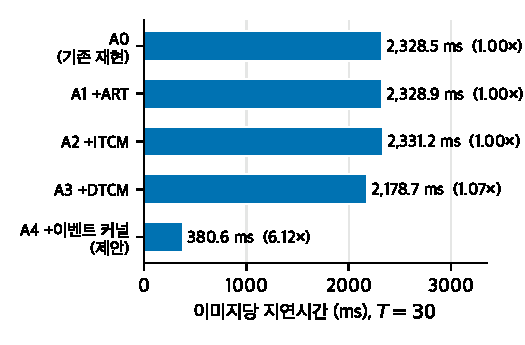
\includegraphics[width=0.92\linewidth]{figures/fig_ablation.pdf}
\caption{누적 절제별 이미지당 지연시간. A1(ART)$\cdot$A2(ITCM)는
0\%, A3(DTCM) 7\%, A4(희소 커널)가 6.12$\times$를 만든다.}
\label{fig:ablation}
\end{figure}

\subsection{레이어 분해}

그림~\ref{fig:layers}은 A0$\cdot$A3$\cdot$A4의 레이어 분해다. 희소
커널의 이득은 발화율이 낮을수록 크다(상한은 발화율의 역수):
밀도 4.1\%인 CPL2는
$1{,}719.8\rightarrow132.2$ms(\textbf{13.0배}), 밀도 47.7\%인 CPL1은
$401.8\rightarrow222.1$ms(1.8배)다. 그 결과 병목의 자리가 바뀌어,
최종 프로파일에서는 CPL1이 전체의 58\%를 차지하는 최대 항목이 된다.
인코딩은 임계값 LUT 캐시(동일 파라미터면 재계산 생략, 비트 불변)로
$35.4\rightarrow5.9$ms가 되었다.

\begin{figure}[htbp]
\centering
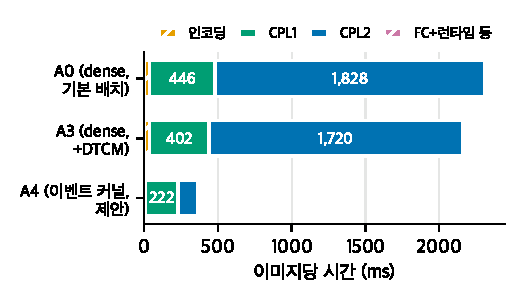
\includegraphics[width=0.95\linewidth]{figures/fig_layers.pdf}
\caption{레이어 분해. 희소 커널(A4)의 이득은 발화율이 낮을수록 크다
--- CPL2(밀도 4.1\%) 13.0$\times$, CPL1(밀도 47.7\%) 1.8$\times$.}
\label{fig:layers}
\end{figure}

\subsection{TFLM 런타임 오버헤드}

동일 최적화를 TFLM 없이 직접 호출하는 A4$'$는 $372.8$ms로, TFLM
경로와의 차이는 이미지당 $7.8$ms(2.1\%)다. 절대치는 선행 연구의
$11.5$ms와 같은 수준이며, 분모(추론 시간)가 6분의 1로 줄면서
비율만 0.5\%에서 2.1\%로 올랐다. 해석기 기반 런타임의 비용은
$T{=}30$회의 Invoke 반복에서도 여전히 수용 가능한 수준이다.
특기할 점은 두 경로의 LIF1 스파이크 진폭이 다름에도(직접 경로
$S_1{=}16{,}384$, TFLM 경로 $32{,}767$ --- 배율은 requantize 계수에
흡수) 출력 체크섬까지 일치한다는 것으로, 퓨전 정수 파이프라인의
일관성에 대한 독립 증거다.

\subsection{비트 동일성 검증}\label{sec:checksum}

회귀 판정은 출력 스파이크 체크섬으로 한다: 매 타임스텝 10개 출력
스파이크 값을 부호 없는 16비트로 누적한 합(8장$\times$30스텝
$\times$10출력, $2{,}400$개 값)이다. 단순한 합이지만 민감도는 높다 ---
LIF는 막전위가 30스텝에 걸쳐 누적되는 상태 기계라서, 네트워크
어디서든 중간값이 1 LSB만 달라져도 발화 타이밍이 바뀌고 그 차이가
다음 레이어$\cdot$다음 스텝으로 연쇄되어 출력 패턴이 달라진다.

실측 결과, \textbf{A0--A4의 다섯 변형과 A4$'$까지 여섯 빌드의
체크섬이 전부 동일}했고(0x00E9FE2C) 8장의 예측도 전부
일치했다(7/8 정답; 표본 8장은 데모 규모로 정확도 지표가 아니다).
dense SMLALD 경로와 무곱셈 희소 경로, 두 실행 경로, 다섯 메모리
배치가 같은 정수 출력을 냄이 실리콘에서 확인된 것이다. 한계도
명시한다: 단순 합이라 오류의 상쇄 우연이 이론상 가능하고, 검증
범위는 8장$\times$30스텝이 실행한 경로다. 전자는 예측 8건의 일치가,
후자는 \ref{sec:identity}절의 구성적 논증이 보완한다. 선행
연구의 호스트 검증(LIF SIMD $1{,}887$만 조합 전수 비교
포함)\cite{cha2026fusion}은 dense 경로 자체의 정당성을 담보한다.

\subsection{메모리 사용}

최종 빌드(A4)의 정적 사용량은 RAM $283{,}072$B(가중치 사본
154KB$+$아레나 64KB 설정 포함), Flash $296{,}432$B이다. TCM 사용은
표~\ref{tab:placement}와 같다(DTCM 89\%, ITCM 30\%). 아레나 실사용은
LIF 상태$\cdot$스크래치의 DTCM 이전으로 $79{,}764$B에서
$25{,}940$B로 줄었다. 가중치 원본 flatbuffer는 플래시에 남아 사본의
원천이 되므로, 순 RAM 비용은 전치 사본 $154{,}368$B와 DTCM
상주분이다. 이 예산은 320KB SRAM 안에서 링크 타임 ASSERT로
강제된다.
